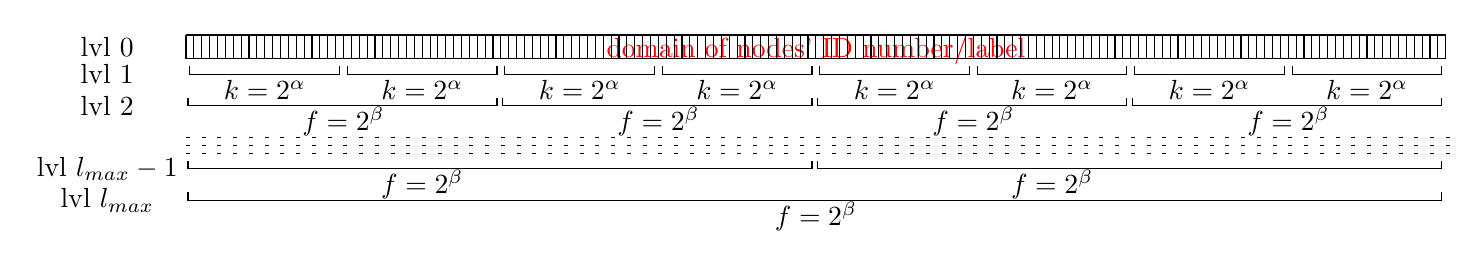
\begin{tikzpicture}

\draw (0,0) -- (16,0) -- (16, -0.3) -- (0, -0.3) -- (0,0);
\node[draw=none, red] at (8, -0.2) {domain of nodes' ID number/label};
\node[draw=none] at (-1, -0.15) {lvl 0};

\foreach \i in {0.1,0.2,...,15.9} {
    \draw (\i,0) -- (\i, -0.3); 
}

\node[draw=none] at (-1, -0.5) {lvl 1};
\foreach \i in {0,2,...,14} {
  \draw (\i + 0.05, -0.4) -- (\i + 0.05, -0.5) -- (\i + 1.95, -0.5) -- (\i + 1.95, -0.4);
  \node[draw=none] at (\i + 1, -0.7) {$k = 2^{\alpha}$};
}

\node[draw=none] at (-1, -0.9) {lvl 2};
\foreach \i in {0,4,8,12} {
  \draw (\i + 0.025, -0.8) -- (\i + 0.025, -0.9) -- (\i + 3.95, -0.9) -- (\i + 3.95, -0.8);
  \node[draw=none] at (\i + 2, -1.1) {$f=2^{\beta}$};
}

\foreach \i in {0,0.2,0.4,...,16} {
  \draw (\i,-1.3) -- (\i+0.05, -1.3) ;
  \draw (\i,-1.4) -- (\i+0.05, -1.4) ;
  \draw (\i,-1.5) -- (\i+0.05, -1.5) ;
}

\node[draw=none] at (-1, -1.7) {lvl $l_{max}-1$};
\foreach \i in {0,8} {
  \draw (\i + 0.025, -1.6) -- (\i + 0.025, -1.7) -- (\i + 7.95, -1.7) -- (\i + 7.95, -1.6);
  \node[draw=none] at (\i + 3, -1.9) {$f=2^{\beta}$};
}

\node[draw=none] at (-1, -2.1) {lvl $l_{max}$};
\draw (0.025, -2) -- (0.025, -2.1) -- (15.95, -2.1) -- (15.95, -2);
\node[draw=none] at (8, -2.3) {$f=2^{\beta}$};

\end{tikzpicture}